\chapter{Preliminaries}
\section{MEMS Microphones}
\label{sec:mems_microphones}
\acrfull{mems} microphones represent a significant evolution in acoustic technology.
Unlike traditional microphones that rely on larger, more mechanically complex systems,
\acrshort{mems} microphones integrate acoustic sensing elements with electronic circuits on a tiny silicon chip.
These microphones have gained immense popularity due to their compact size, robustness, and cost-effectiveness.
\acrshort{mems} technology allows for the production of microphones with high sound quality and excellent reliability,
making them ideal for a wide range of applications including mobile devices, wearable technology, and \acrshort{iot} devices.
Their small footprint also enables design flexibility in increasingly miniaturized electronic devices.
\acrshort{mems} microphones differ in their output signal types, leading to three categories: analog microphones, \acrshort{pdm} microphones, and \acrshort{pcm} microphones.
\begin{figure}[h]
	\centering
	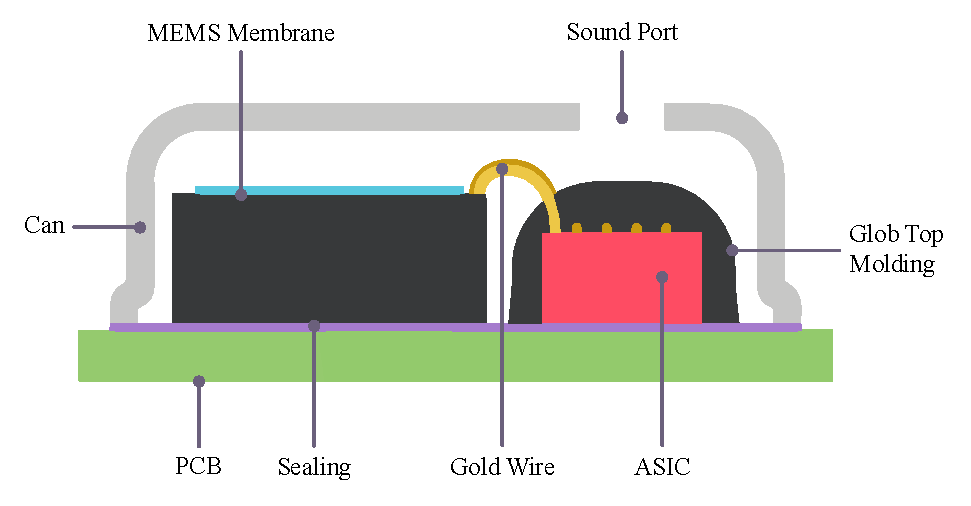
\includegraphics[width=0.9\textwidth]{images/2_preliminaries/mems_microphone_illustration.pdf}
	\caption{Internal Structure of a MEMS Microphone \cite{mems_microphone_construction}}
	\label{fig:mems_microphone}
\end{figure}

\subsection{Analog Microphones} \label{sec:analog_microphones}
Analog \acrshort{mems} microphones convert sound into an analog electrical signal.
They are simple and easy to integrate in analog circuits but may require additional signal amplification components.
A disadvantage of analog microphones is that they are susceptible to noise and interference, making them unsuitable for long-distance transmission.
\begin{figure}[h!]
	\centering
	\vspace{-0.1cm}
	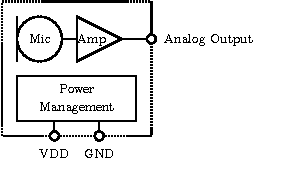
\includegraphics[height=2.9cm, trim={0 0.4cm 0 0}]{images/2_preliminaries/mems_microphone_types_analog.pdf}
	\caption{Block Diagram of analog MEMS Microphone}
	\label{fig:mems_microphone_types_analog}
\end{figure}

\subsection{PDM Microphones} \label{sec:pdm_microphones}
\acrshort{pdm} microphones output a digital signal representing the acoustic waveform.
Their digital format is noise-resistant and supports long-distance transmission, making them ideal for multiplexed, multi-microphone setups.
These microphone types require a high-frequency clock signal to operate (typically 1.5\,MHz to 3.25\,MHz),
which must be provided by the host (e.g. a \acrshort{mcu} or \acrshort{fpga}).
A dedicated channel select pin is used to select the microphone's output channel in multiplexed systems.
\begin{figure}[h!]
	\centering
	\vspace{-0.1cm}
	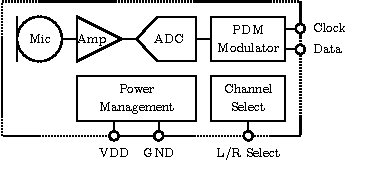
\includegraphics[height=2.9cm, trim={0 0.4cm 0 0}]{images/2_preliminaries/mems_microphone_types_pdm.pdf}
	\caption{Block Diagram of PDM MEMS Microphone}
	\label{fig:mems_microphone_types_pdm}
\end{figure}

\subsection{PCM Microphones} \label{sec:pcm_microphones}
\acrshort{pcm} microphones provide a digital output using the \acrlong{pcm} format, most often interfaced via the \acrshort{i2s} protocol.
Compared to \acrshort{pdm} microphones, \acrshort{pcm} microphones have a build-in decimation filter, which simplifies the signal processing chain, as the host no longer needs to perform this task.
However, \acrshort{pcm} microphones are more complex, costly and less common in the industry than \acrshort{pdm} microphones.
\begin{figure}[h!]
	\centering
	\vspace{-0.1cm}
	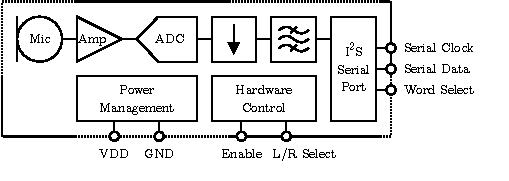
\includegraphics[height=2.9cm, trim={0 0.4cm 0 0}]{images/2_preliminaries/mems_microphone_types_pcm.pdf}
	\caption{Block Diagram of PCM MEMS Microphone}
	\label{fig:mems_microphone_types_pcm}
\end{figure}
\clearpage

\subsection{Microphone Port Location}
\acrshort{mems} microphones can be categorized based on their port location: top-port and bottom-port.
Top-port microphones have the sound inlet on the top of the package, suitable when the sound source is above the microphone.
Conversely, bottom-port microphones have the inlet at the bottom, ideal for mounting on surfaces where sound comes from the side or below.
For bottom-port microphones, the sound must travel through a hole in the \acrshort{pcb} to reach the microphone, which can affect the sound quality.
\begin{figure}[h!]
	\centering
	\begin{minipage}{0.49\textwidth}
		\centering
		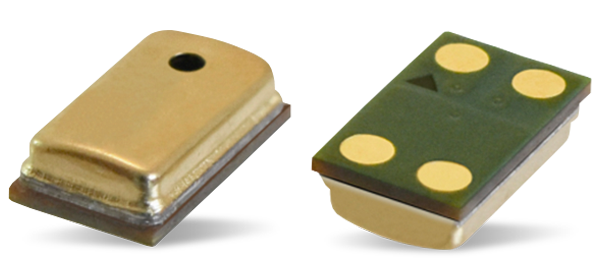
\includegraphics[width=\textwidth]{images/2_preliminaries/mems_microphone_top.png}
		\caption{Top-Port MEMS Microphone}
		\label{fig:mems_microphone_top}
	\end{minipage}
	\begin{minipage}{0.49\textwidth}
		\centering
		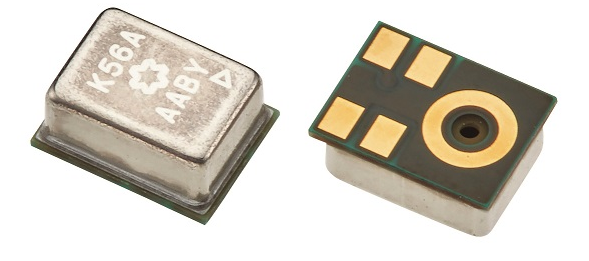
\includegraphics[width=\textwidth]{images/2_preliminaries/mems_microphone_bottom.png}
		\caption{Bottom-Port MEMS Microphone}
		\label{fig:mems_microphone_bottom}
	\end{minipage}
\end{figure}


\section{Pulse Density Modulation (PDM)}
\acrfull{pdm} is a modulation technique used to represent an analog signal with a binary sequence.
In \acrshort{mems} microphones, the diaphragm movements modulate a high-frequency carrier signal,
resulting in a digital output where the density of pulses corresponds to the amplitude of the input signal.
\acrshort{pdm} simplifies the microphone design, allowing for smaller and more power-efficient devices.
However, it requires a decimation filter in the signal processing chain to convert the high-frequency pulse sequence into a usable digital audio signal.
The \acrshort{pdm} bitstream is encoded from an analog signal through the process of 1-bit delta-sigma (\(\Delta \Sigma\)) modulation.
This process uses a one-bit quantizer that outputs either a 1 or 0 depending on the amplitude of the analog signal.
Due to the nature of real-world analog signals, a quantization error occurs, representing the difference between the 1 or 0 and the actual amplitude it represents.
This error is negatively fed back in the \(\Delta \Sigma\) process loop, influencing every subsequent quantization measurement and its error.
This feedback mechanism averages out the quantization error, enhancing the accuracy of the \acrshort{pdm} representation.
\begin{figure}[h]
	\centering
	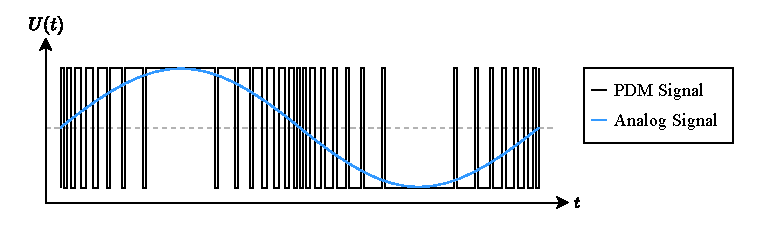
\includegraphics[width=1.0\textwidth]{images/2_preliminaries/pdm_modulation.pdf}
	\caption{PDM Modulation Example}
	\label{fig:pdm_modulation}
\end{figure}


\section{Time Division Multiplexing (TDM)}
\acrfull{tdm} is a method of transmitting and receiving independent signals over a common signal path by means of synchronized switches at each end of the transmission line.
In the context of digital audio, \acrshort{tdm} allows multiple audio streams to share a single communication line,
with each stream getting a dedicated time slot. This technique is valuable in systems where multiple audio channels,
such as in surround sound systems or multi-microphone arrays, need to be transmitted over a single cable.
\acrshort{tdm}'s main advantage is its ability to efficiently handle multiple audio streams without the need for multiple physical connections.
This makes it particularly useful in professional audio applications, broadcast systems, and complex audio setups.
However, \acrshort{tdm} systems can be more complex to implement and require precise synchronization to ensure that the timing of the different channels is maintained.
Figure \ref{fig:tdm_example} shows an example of a TDM-16 system with 16 bits sample width.
\begin{figure}[h]
	\centering
	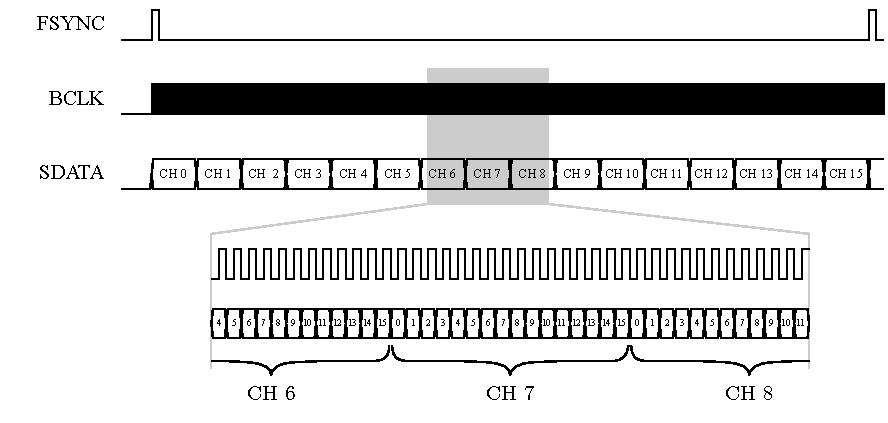
\includegraphics[width=1.0\textwidth, trim={0.5cm 0 0 0}]{images/2_preliminaries/tdm_signals.pdf}
	\caption{Example of TDM-16 with 16 bits sample width}
	\label{fig:tdm_example}
\end{figure}

\acrfull{tdm} systems introduces tristate outputs, enabling multiple devices to share the same physical bus without interference.
The \acrshort{tdm} bus consists of three signals: \textit{fsync}, \textit{bclk} and \textit{data}.
\begin{itemize}
	\item \textbf{FSYNC (Frame Sync)}: This signal marks the start of a frame in the TDM stream.
	      It acts as a reference point for aligning the data across all channels.
	      In a TDM-16 system, FSYNC indicates the beginning of a sequence of 16 channels (slots).
	\item \textbf{BCLK (Bit Clock)}: This clock signal dictates the timing for data transmission.
	      Each edge of the BCLK corresponds to a bit position in the data stream.
	      For 16-bit samples, there are 16 BCLK pulses per channel, hence 256 BCLK pulses per frame.
	\item \textbf{Data}: The actual audio data is transmitted in a series of bits.
	      In a 16-channel, 16-bit TDM system, each channel's data is represented by 16 bits (Left Justified).
\end{itemize}


\section{GNSS Real-Time Kinematic (RTK)}
The \acrfull{gnss} \acrfull{rtk} is an advanced technique used in geodesy and navigation
that enhances the precision of position data derived from satellite-based positioning systems.
\acrshort{rtk} uses differential techniques to improve the accuracy of position information obtained from satellite systems like
\acrshort{gps}, GLONASS, Galileo, or BeiDou.
This method is particularly useful in applications requiring high precision,
such as surveying, construction, and precision agriculture.

\subsection{Custom Node as an Anchor}
One method to utilize \acrshort{rtk} for achieving enhanced position accuracy involves using a custom node as an anchor.
This method requires setting up a fixed \acrshort{rtk} base station at a known location.
The base station calculates error values for satellite signals by comparing the expected signal (based on its known location) with the received signal.
These error values, which account for various factors like atmospheric interference and satellite orbit errors,
are then transmitted to a mobile \acrshort{rtk} receiver.
The mobile receiver uses these corrections to adjust its own satellite signal measurements, significantly improving its positional accuracy.

\subsection{Using Data from a Public Provider}
Alternatively, \acrshort{rtk} corrections can be obtained from a public provider.
In this approach, the user does not set up a custom anchor node but instead subscribes to a service that provides \acrshort{rtk} correction data.
These services operate a network of \acrshort{rtk} base stations and compute correction factors for different regions.
The correction data is typically transmitted via the internet directly to the user's \acrshort{rtk} receiver.
This method is convenient for users who do not have the resources to establish and maintain their own \acrshort{rtk} base station.
By applying these corrections, which include compensating for atmospheric drift and other errors,
the user's receiver can achieve a similar level of enhanced positional accuracy as with a custom anchor node.
